\documentclass[sigconf]{acmart}
\usepackage{balance}

\usepackage{listings}
\usepackage{xcolor}

\settopmatter{printacmref=false}
\renewcommand\footnotetextcopyrightpermission[1]{}
\acmConference[HPC UniSa course]{High Performace Computing course}{2025}{Fisciano, Italy}


\lstdefinelanguage{cudaerror}{
  morekeywords={UR, CUDA, ERROR},
  sensitive=false,
}

\lstdefinestyle{errorlog}{
  basicstyle=\ttfamily\footnotesize,
  backgroundcolor=\color{gray!10},
  frame=single,
  breaklines=true,
  postbreak=\mbox{\textcolor{red}{$\hookrightarrow$}\space},
  keywordstyle=\color{red!70!black}\bfseries,
}

% bold paragraph titles
\newcommand{\mypar}[1]{{\bf #1.}}

% Metadata
\title{Extending and Reproducing pSTL-Bench: oneDPL Backend Integration and Enhanced Reproducibility}

\author{Oleg Bilovus}
\affiliation{
  \institution{Department of Computer Science, University of Salerno}
  \city{Fisciano (SA)}
  \country{Italy}
}

\balance{}
\begin{document}

\begin{abstract}
      Describe in concise words what you do, why you do it (not necessarily
      in this order), and the main result.  The abstract has to be
      self-contained and readable for a person in the general area. You
      should write the abstract last.
\end{abstract}

\maketitle

\section{Introduction}\label{sec:intro}
Writing performance-portable and efficient parallel applications remains a
significant challenge due to the diversity of modern hardware architectures.
The emergence of parallel programming frameworks and, more recently, the
introduction of parallel algorithms in the \textit{C++17 Standard Template
      Library (STL)} aim to address this challenge by enabling developers to write
code that runs efficiently across CPUs and GPUs using a standardized interface.

\textit{pSTL-Bench}~\cite{pSTL-Bench} is a benchmark suite originally developed to
quantitatively evaluate the performance of individual parallel STL algorithms
across various compiler frameworks (such as GCC, Intel's icpx, NVIDIA HPC SDK)
and backends (including TBB, HPX, OpenMP, and CUDA). It provides a focused,
micro-benchmarking approach that avoids the complexities of full applications
and highlights the relative performance characteristics of different STL
implementations.

\mypar{This Work} In this work, the main results and experiments from the original pSTL-Bench
paper are reproduced. Beyond reproduction, the project is then extended by
incorporating support for the \textit{oneAPI DPC++ Library (oneDPL)} backend,
enabling the evaluation of Intel’s parallel STL implementation based on the
\textit{SYCL programming model} on both CPU and GPU platforms

To further enhance the usability and reproducibility of the benchmark suite,
automation tools are introduced, including Ansible playbooks for environment
setup and benchmark execution, R scripts for performance analysis, and expanded
documentation for ease of deployment and adding new backends.

\mypar{Related Work} This work builds directly on pSTL-Bench.
While performance portability and parallelism have been widely studied in
the context of full applications~\cite{app} and frameworks such as Kokkos~\cite{Kokkos}
and RAJA~\cite{RAJA}, no prior work has reproduced or extended pSTL-Bench,
nor added support for the oneDPL backend or focused on improving its reproducibility.

\section{Background}\label{sec:background}
This section introduces the relevant concepts and context for evaluating the
scalability of parallel algorithms implemented in the C++ Standard Template
Library (STL). It defines the scope of the problem, outlines the algorithms
under analysis, and describes the supporting frameworks and benchmarking
strategies used for performance assessment.

\mypar{Parallel STL in C++} Since C++17, the Standard Template Library (STL) includes parallel versions
of many common algorithms, enabling hardware parallelism through
familiar interfaces. Compiler support varies, relying on different
runtimes and libraries to target platforms such as multi-core CPUs
and GPUs, with differences in scheduling, memory use, and synchronization.

\mypar{Problem Definition} The primary objective is to analyze how different implementations
of parallel STL algorithms scale with increasing problem sizes and hardware resources.
This includes identifying the computational overheads and the performance gains achieved
through parallel execution. A detailed performance comparison is necessary to understand
which combinations of compilers and backends provide the most efficient use of available
computing resources.

\mypar{Algorithms} The study focuses on five representative algorithms that embody diverse computational patterns:
\begin{itemize}
      \item \textbf{find} – Searches for a target value within a range using linear traversal.
      \item \textbf{for\_each} – Executes a loop with $k_{it}$ increments per element to simulate computation and stores the result.
            $k_{it}$ is a parameter that can be adjusted to control the workload.
      \item \textbf{inclusive\_scan} – Produces a prefix sum, where each element in the output is the sum of all previous elements
            plus the current element, requiring synchronization.
      \item \textbf{reduce} – Computes a single result by summing all elements in a range, which can be parallelized
            but requires synchronization to combine results.
      \item \textbf{sort} – Rearranges elements into ascending order, requiring synchronization and data movement.
\end{itemize}

\mypar{Backends} In this work, support for the \textit{oneAPI DPC++ Library (oneDPL)} is added, which is based on the SYCL
programming model and enables parallel STL execution on both CPUs and GPUs.

The original pSTL-Bench suite includes the following backends:
\begin{itemize}
      \item \textbf{GNU Parallel STL} – The GCC implementation of parallel algorithms using OpenMP.
      \item \textbf{TBB} – A C++ library offering task-based parallel algorithms and data structures.
      \item \textbf{HPX} – A C++ runtime for fine-grained parallel and distributed applications.
      \item \textbf{OpenMP} – A standard API for shared-memory parallel programming.
      \item \textbf{CUDA} – NVIDIA’s platform for general-purpose GPU computing.
\end{itemize}

The evaluation covers various compiler-backend combinations, including those
based on GNU, Intel, and NVIDIA compilers.

\mypar{Automation} To facilitate reproducibility and ease of use, the project includes automation tools:
\begin{itemize}
      \item \textbf{Ansible} – An agentless automation tool that simplifies the setup of the benchmark environment,
            including installation of dependencies, configuration of the system, compilation of the benchmark suite, and execution of tests.
      \item \textbf{Semaphore UI} – A web-based interface for managing and monitoring the execution of ansible playbooks,
            providing a user-friendly way to trigger tests and view results.
      \item \textbf{R Scripts} – Scripts for analyzing performance data, generating plots similar to those in the original paper.
            and providing insights into the performance characteristics of different implementations.
\end{itemize}

\section{Benchmark Setup}\label{sec:benchmark_setup}

This section describes the hardware and software setup used for the
benchmarking experiments, including platform specifications, compiler versions,
and the configuration of the parallel STL implementations.

\mypar{Hardware Platform}
The benchmarks were executed on a \textit{DELL G16 7630} laptop connected to external power,
with the hardware specifications shown in Table~\ref{tab:hardware-config}.

\begin{table}[h]
      \centering
      \caption{Hardware configuration}\label{tab:hardware-config}
      \begin{tabular}{|l|l|}
            \hline
            \multicolumn{2}{|c|}{\textbf{CPU}~\cite{cpu_specs}} \\
            \hline
            Processor      & Intel Core i9-13900HX              \\
            Cores          & 24 (8 P-cores + 16 E-cores)        \\
            Core Frequency & 2.20 GHz (up to 5.40 GHz)          \\
            Threads        & 32 threads                         \\
            Memory         & 32 GB RAM                          \\
            \hline
            \hline
            \multicolumn{2}{|c|}{\textbf{GPU}~\cite{gpu_specs}} \\
            \hline
            GPU            & NVIDIA GeForce RTX 4070 (mobile)   \\
            CUDA Cores     & 4608 CUDA cores                    \\
            Core Frequency & 1230 MHz (up to 2175 MHz)          \\
            Memory         & 8 GB GDDR6 VRAM                    \\
            \hline
      \end{tabular}
\end{table}

\mypar{Software Platform}
The benchmarks were executed on a Linux-based operating system, specifically \textit{Ubuntu 25.04 Desktop}.
The desktop version was used due to GPU driver compatibility issues with the server edition. Prior to execution,
the CPU frequency governor was set to \textit{performance} mode to ensure maximum processor performance~\cite{google_benchmark:governor}.

\mypar{Compilers and Libraries}
The compilers and libraries used in the experiments are listed in Table~\ref{tab:compilers} and Table~\ref{tab:libraries}, respectively.

\begin{table}[h]
      \centering
      \begin{minipage}[t]{0.48\linewidth}
            \centering
            \caption{Compilers}\label{tab:compilers}
            \begin{tabular}{|l|l|}
                  \hline
                  \textbf{Compiler} & \textbf{Version} \\
                  \hline
                  g++               & 14.2.0           \\
                  Intel icpx        & 2025.1.1         \\
                  NVIDIA nvc++      & 25.3-0           \\
                  \hline
            \end{tabular}
      \end{minipage}
      \hfill
      \begin{minipage}[t]{0.48\linewidth}
            \centering
            \caption{Libraries}\label{tab:libraries}
            \begin{tabular}{|l|l|}
                  \hline
                  \textbf{Library} & \textbf{Version} \\
                  \hline
                  oneDPL           & 2022.8           \\
                  TBB              & 2022.1           \\
                  HPX              & 1.9.1            \\
                  NVOMP            & 25.3             \\
                  CUDA             & 12.8             \\
                  \hline
            \end{tabular}
      \end{minipage}
\end{table}

\section{Experiment Details}\label{sec:exp_details}
All aspects of the original pSTL-Bench experiments are replicated in this work,
with one exception: the problem size in certain experiments is reduced from
$2^{30}$ to $2^{29}$. This adjustment was necessary due to runtime crashes
encountered by the oneDPL backend when using the larger problem size. The
corresponding error message is shown in Listing~\ref{lst:onedpl-error}.

\begin{lstlisting}[style=errorlog, caption={oneDPL GPU runtime error output}, label={lst:onedpl-error}]
<CUDA>[ERROR]: 
UR CUDA ERROR:
  Value:           2
  Name:            CUDA_ERROR_OUT_OF_MEMORY
  Description:     out of memory
  Function:        allocateMemObjOnDeviceIfNeeded
  Source Location: /builds/oneapi-core/oneapi-release-package/intel-llvm-mirror/build/_deps/unified-runtime-src/source/adapters/cuda/memory.cpp:442

<CUDA>[ERROR]: 
UR CUDA ERROR:
  Value:           2
  Name:            CUDA_ERROR_OUT_OF_MEMORY
  Description:     out of memory
  Function:        allocateMemObjOnDeviceIfNeeded
  Source Location: /builds/oneapi-core/oneapi-release-package/intel-llvm-mirror/build/_deps/unified-runtime-src/source/adapters/cuda/memory.cpp:442

terminate called after throwing an instance of 'sycl::_V1::exception'
  what():  Native API failed. Native API returns: 38 (UR_RESULT_ERROR_OUT_OF_HOST_MEMORY)
\end{lstlisting}

\section{Experimental Results}

This section presents the results of experiments designed to evaluate the
performance of parallel STL algorithms across various compiler-backend
combinations. While each experiment references the original results from the
pSTL-Bench paper, those plots are not reproduced here. Readers are encouraged
to consult the original publication for direct visual comparisons.

All plots presented in this work were generated using the R scripts available
in the forked repository. Figures were exported at a resolution of 300 DPI to
preserve detail and support zooming without quality loss.

The compiler names used in the plots differ from those in the original
pSTL-Bench paper, as they are directly generated by the benchmarking tool.
These names can be mapped to their original counterparts as follows:
\begin{itemize}
      \item \textit{GNU-OMP} corresponds to \textit{GCC-GNU}.
      \item \textit{GNU-*} corresponds to \textit{GCC-*}.
      \item \textit{IntelLLVM-TBB} corresponds to \textit{ICC-TBB}.
      \item \textit{NVHPC-*} corresponds to \textit{NVC-*}.
\end{itemize}

To maintain consistency, the structure and subsection titles align with those
of the original work.

\subsection{The Impact of Memory Allocation}

The first experiment investigates the effect of the custom memory allocator
used in pSTL-Bench on the performance of parallel STL algorithms. Whereas the
original study employed a problem size of $2^{30}$, this setup uses a reduced
size of $2^{29}$, as described in Section~\ref{sec:exp_details}.

In the original paper, the custom allocator demonstrated significant
performance improvements—particularly for the \textit{for\_each} and
\textit{reduce} algorithms—achieving speedups of up to 1.5x over the default
allocator.

In this evaluation, no substantial performance difference was observed between
the custom and default allocators. The measured results are presented in
Figure~\ref{fig:speedup_customAllocator}.

Despite the minimal performance impact in this setting, the custom allocator
was retained to ensure consistency with the methodology of the original study.

\begin{figure}[H]
      \centering
      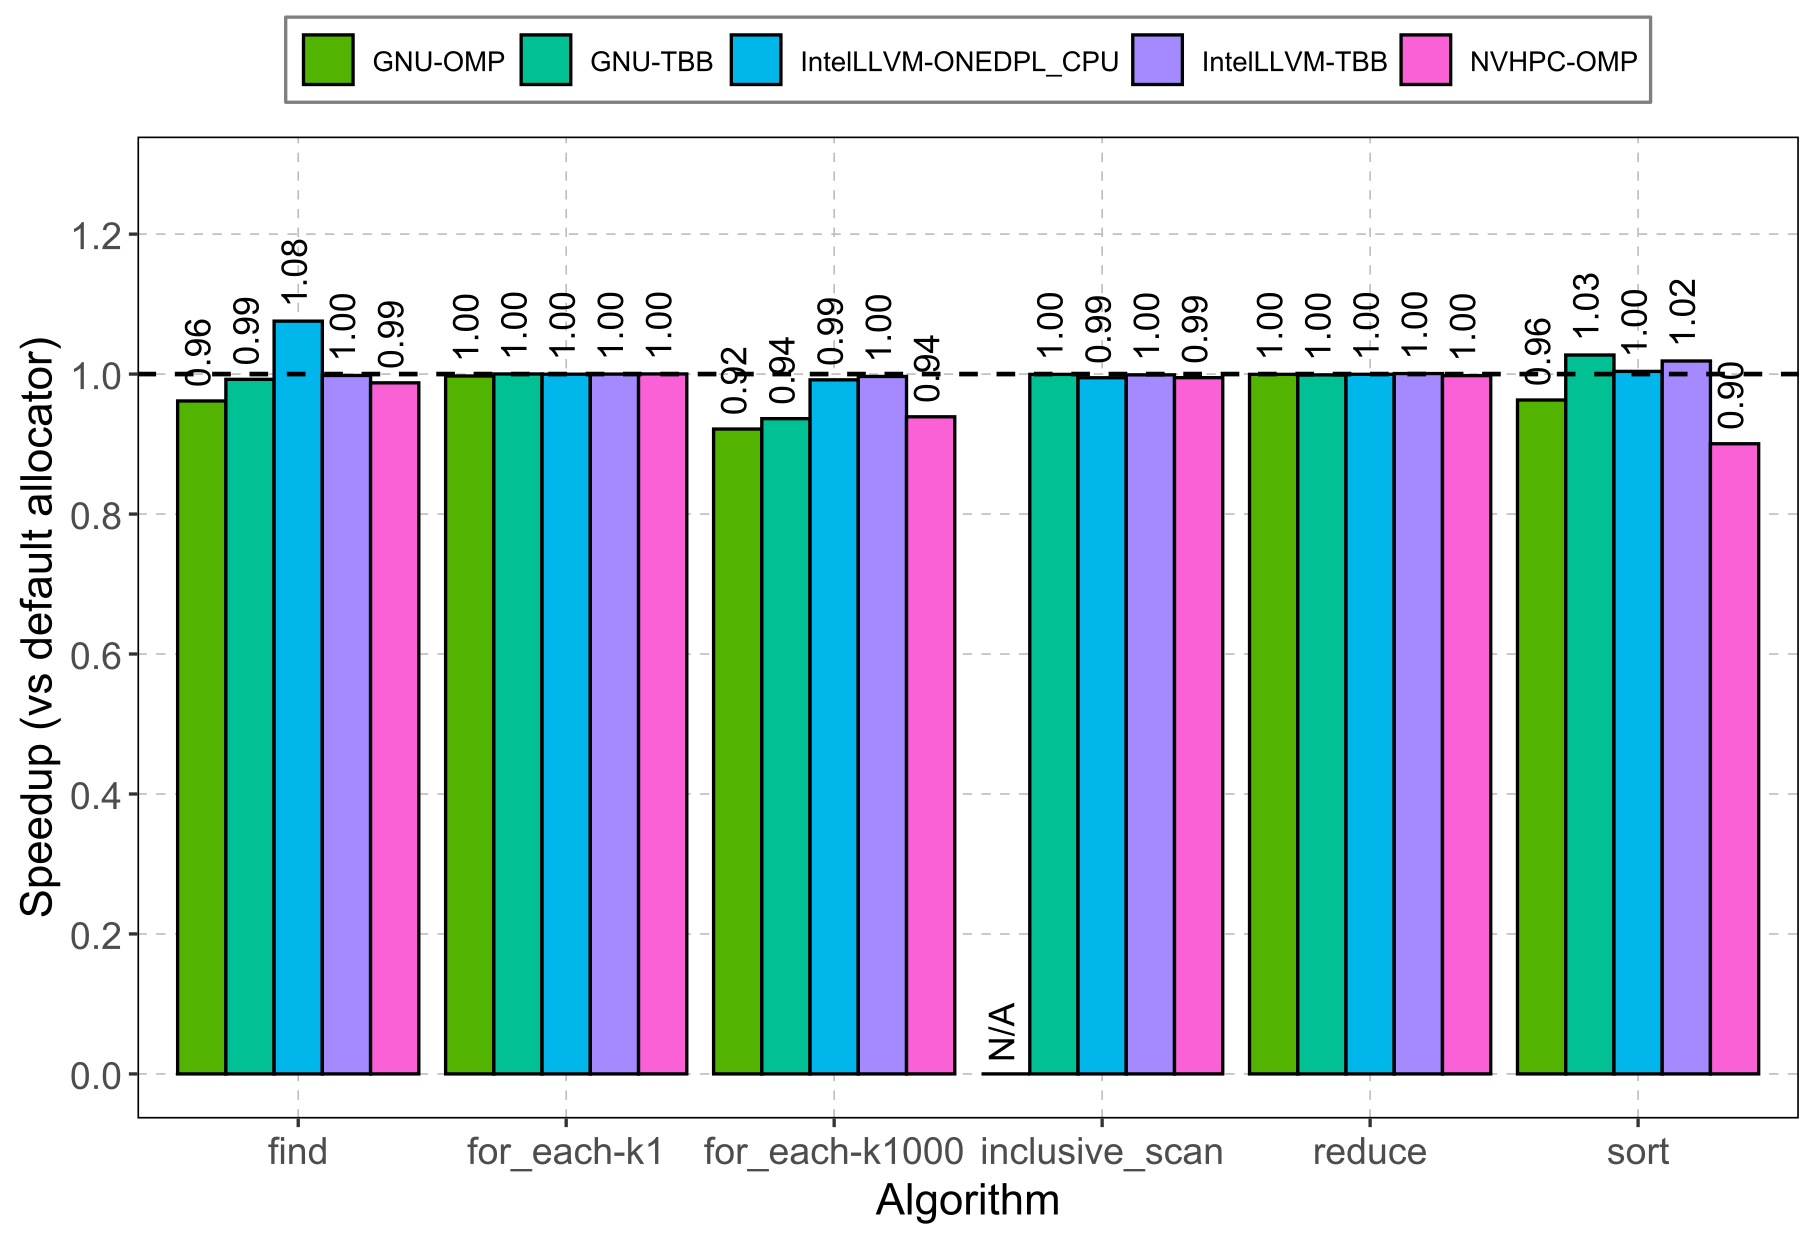
\includegraphics[width=\linewidth]{figures/speedup_customAllocator}
      \caption{Speedup when using custom parallel allocator with 32 threads and a problem size of $2^{29}$. Higher is better.}\label{fig:speedup_customAllocator}
\end{figure}

\subsection{X::for\_each}

This experiment evaluates the performance of the \textit{for\_each} algorithm.
The parameter $k_{it}$ represents the arithmetic intensity of the workload. For
higher values of $k_{it}$, performance is expected to approach ideal speedup.

Figure~\ref{fig:problemSize_time-for_each} presents the execution time for
\textit{for\_each} with minimal and maximal $k_{it}$ values. The results
closely resemble those reported in the original pSTL-Bench paper. For $k_{it} =
      1$, the NVIDIA OpenMP backend achieves the best performance. In contrast, for
$k_{it} = 1000$, all backends exhibit comparable execution times.

The oneDPL backend on CPU consistently performed worse than the other backends
across both configurations.

\begin{figure}[H]
      \centering
      \begin{minipage}[t]{0.48\linewidth}
            \centering
            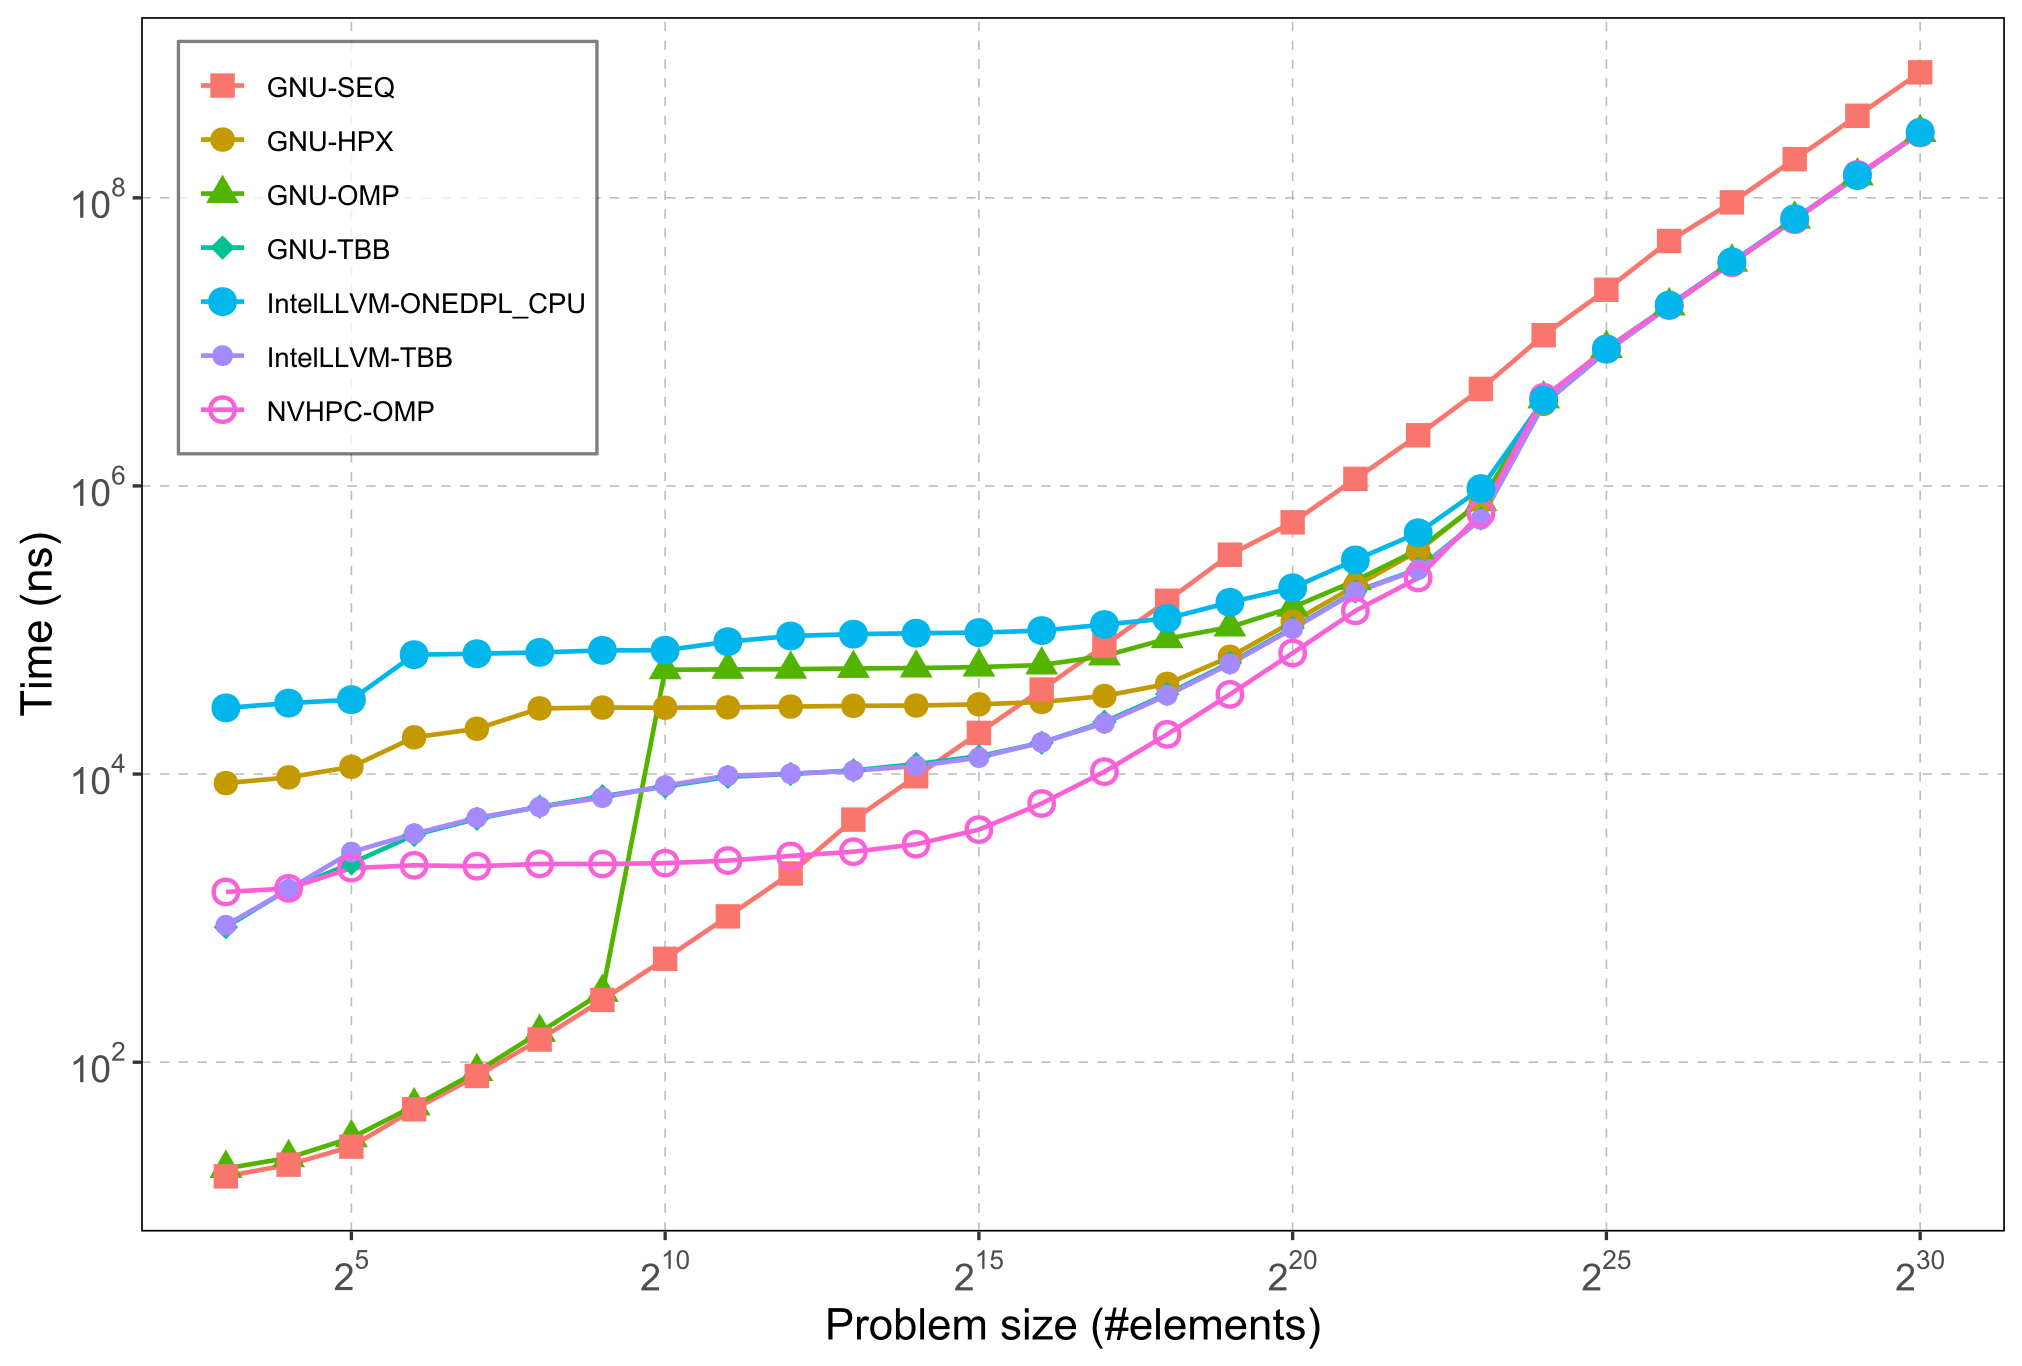
\includegraphics[width=\linewidth]{figures/problemSize_time-for_each-k1.png}
            \caption*{(a) $k_{it} = 1$.}
      \end{minipage}
      \hfill
      \begin{minipage}[t]{0.48\linewidth}
            \centering
            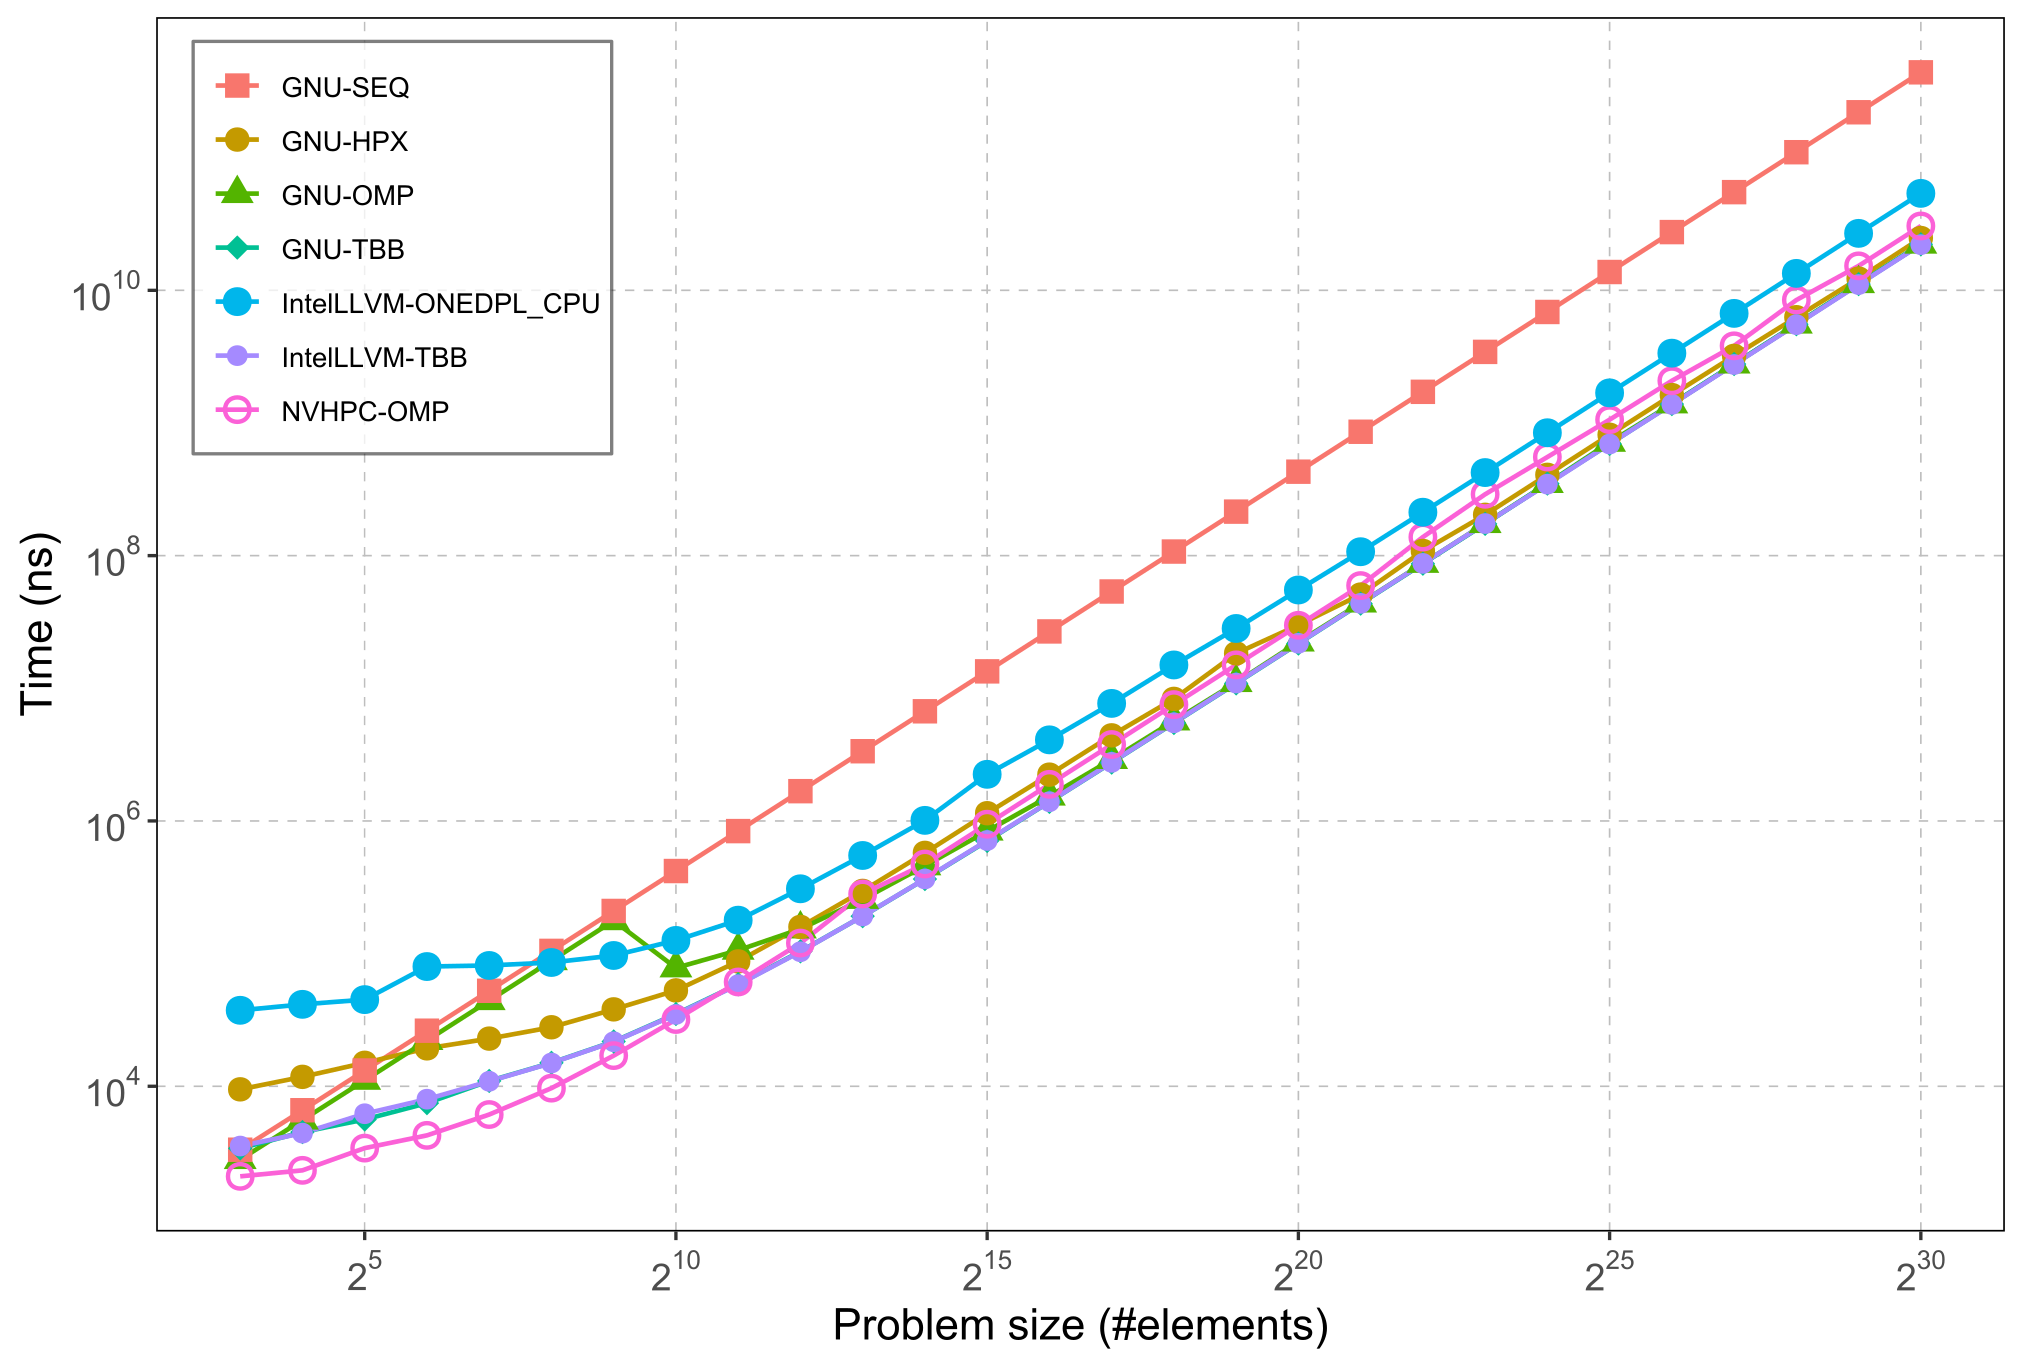
\includegraphics[width=\linewidth]{figures/problemSize_time-for_each-k1000.png}
            \caption*{(b) $k_{it} = 1000$.}
      \end{minipage}
      \caption{Results for benchmark X::for\_each. Problem size scaling using all
            cores except for the GNU-SEQ implementation. Lower is better.}
      \label{fig:problemSize_time-for_each}
\end{figure}

Figure~\ref{fig:speedup_threads-for_each} shows the strong scaling results for
the \textit{for\_each} algorithm with $2^{29}$ elements. Compared to the
original paper, the results differ slightly. In the original study, all
backends achieved ideal speedup for $k_{it} = 1000$ and near-ideal speedup for
$k_{it} = 1$.

In this evaluation, the oneDPL backend on CPU underperforms relative to the
others. Additionally, all backends begin to lose scalability beyond 8 threads,
which is likely due to the hardware architecture—specifically, the presence of
8 performance cores (P-cores) and 16 efficiency cores (E-cores).

\begin{figure}[H]
      \centering
      \begin{minipage}[t]{0.48\linewidth}
            \centering
            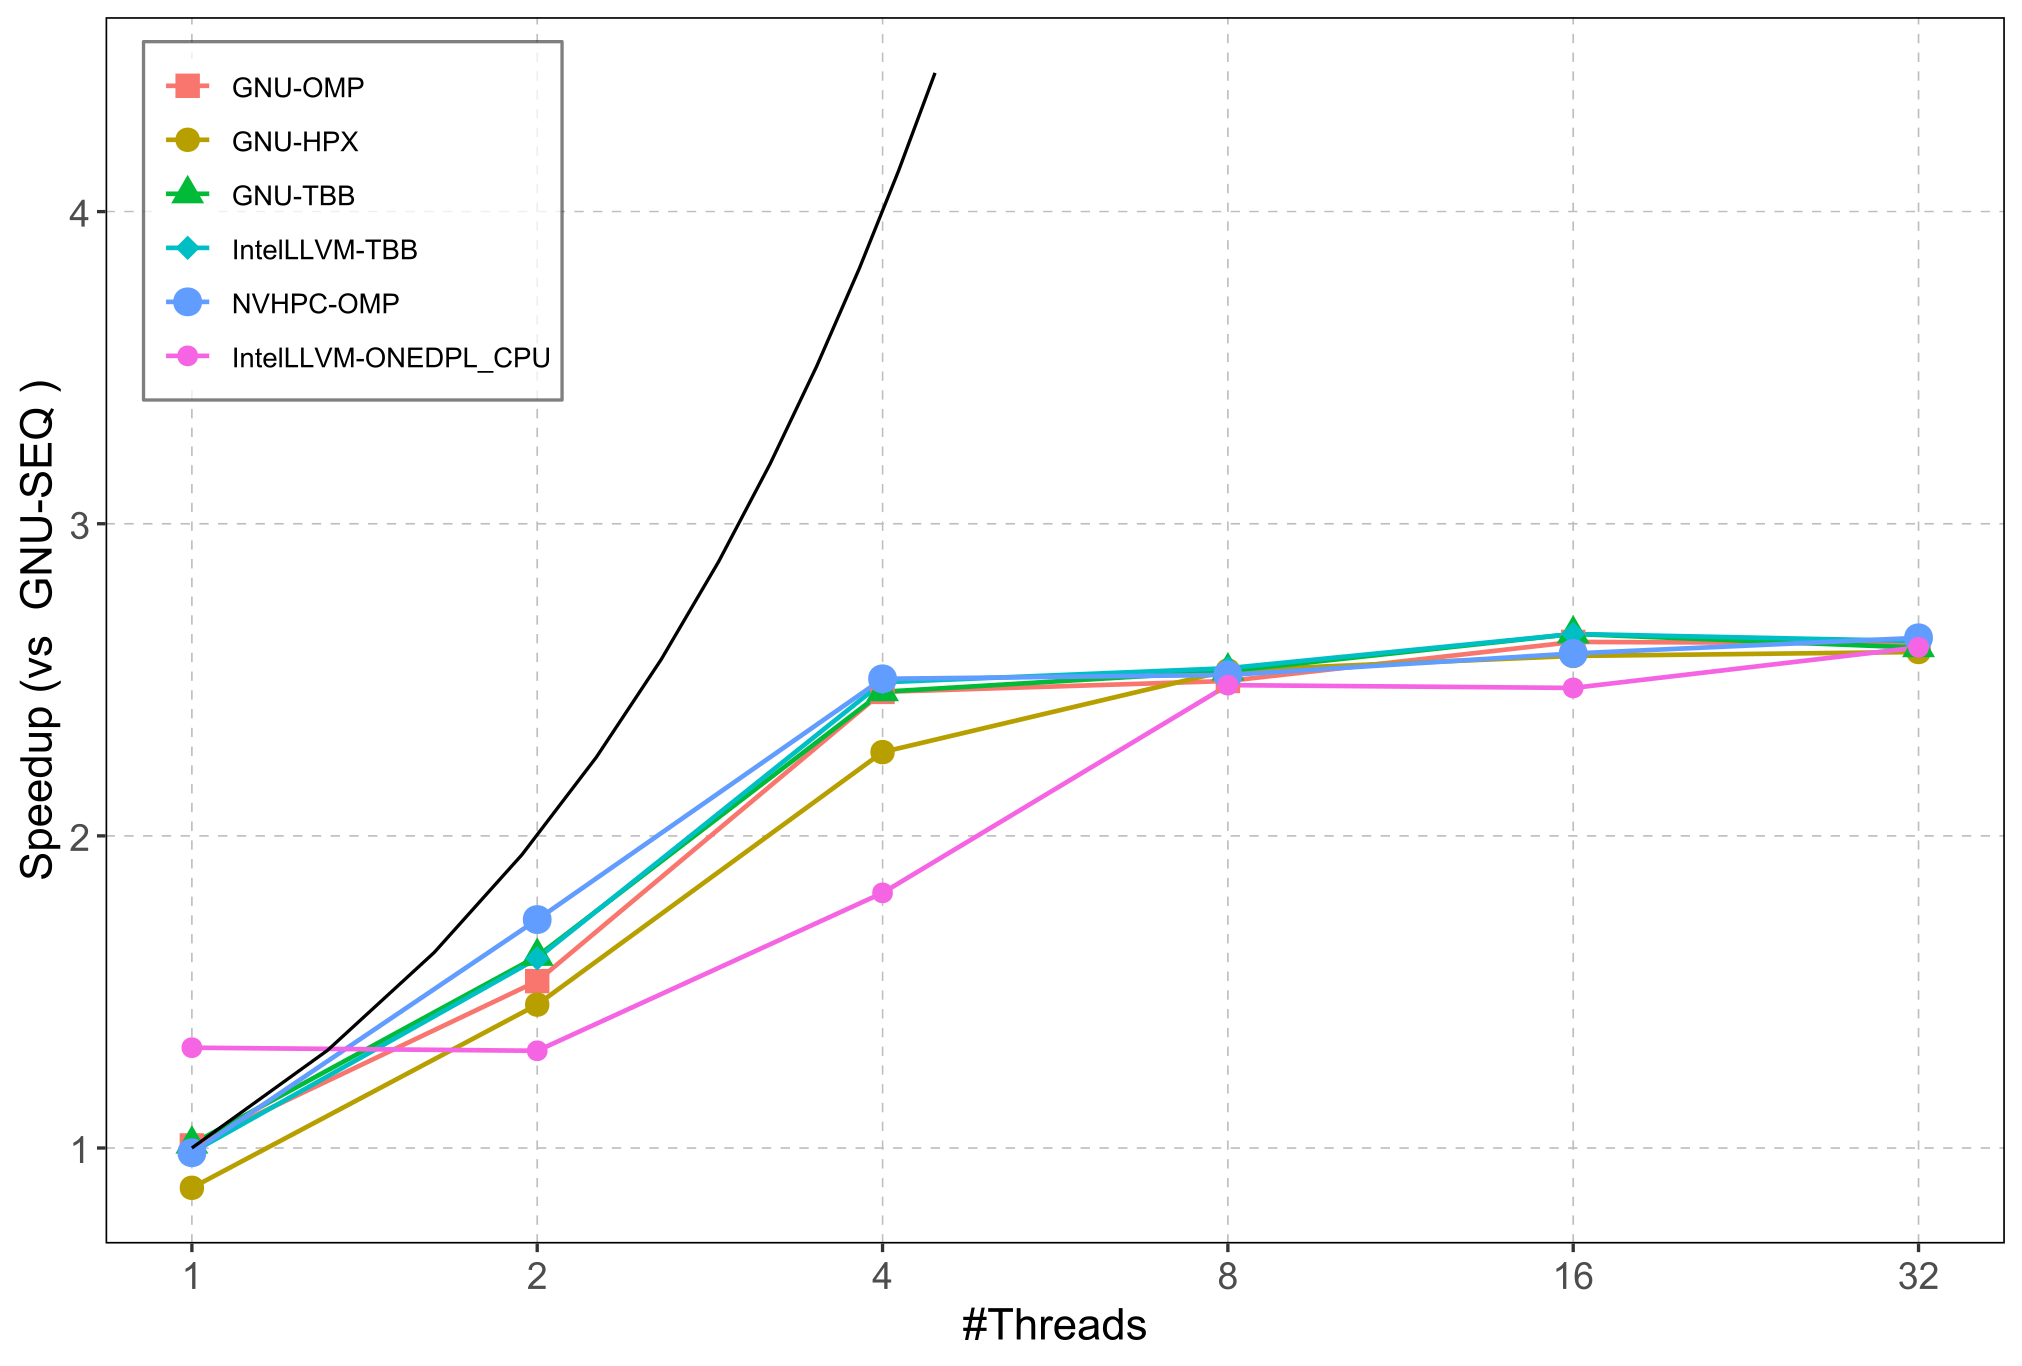
\includegraphics[width=\linewidth]{figures/speedup_threads-for_each-k1.png}
            \caption*{(a) $k_{it} = 1$.}
      \end{minipage}
      \hfill
      \begin{minipage}[t]{0.48\linewidth}
            \centering
            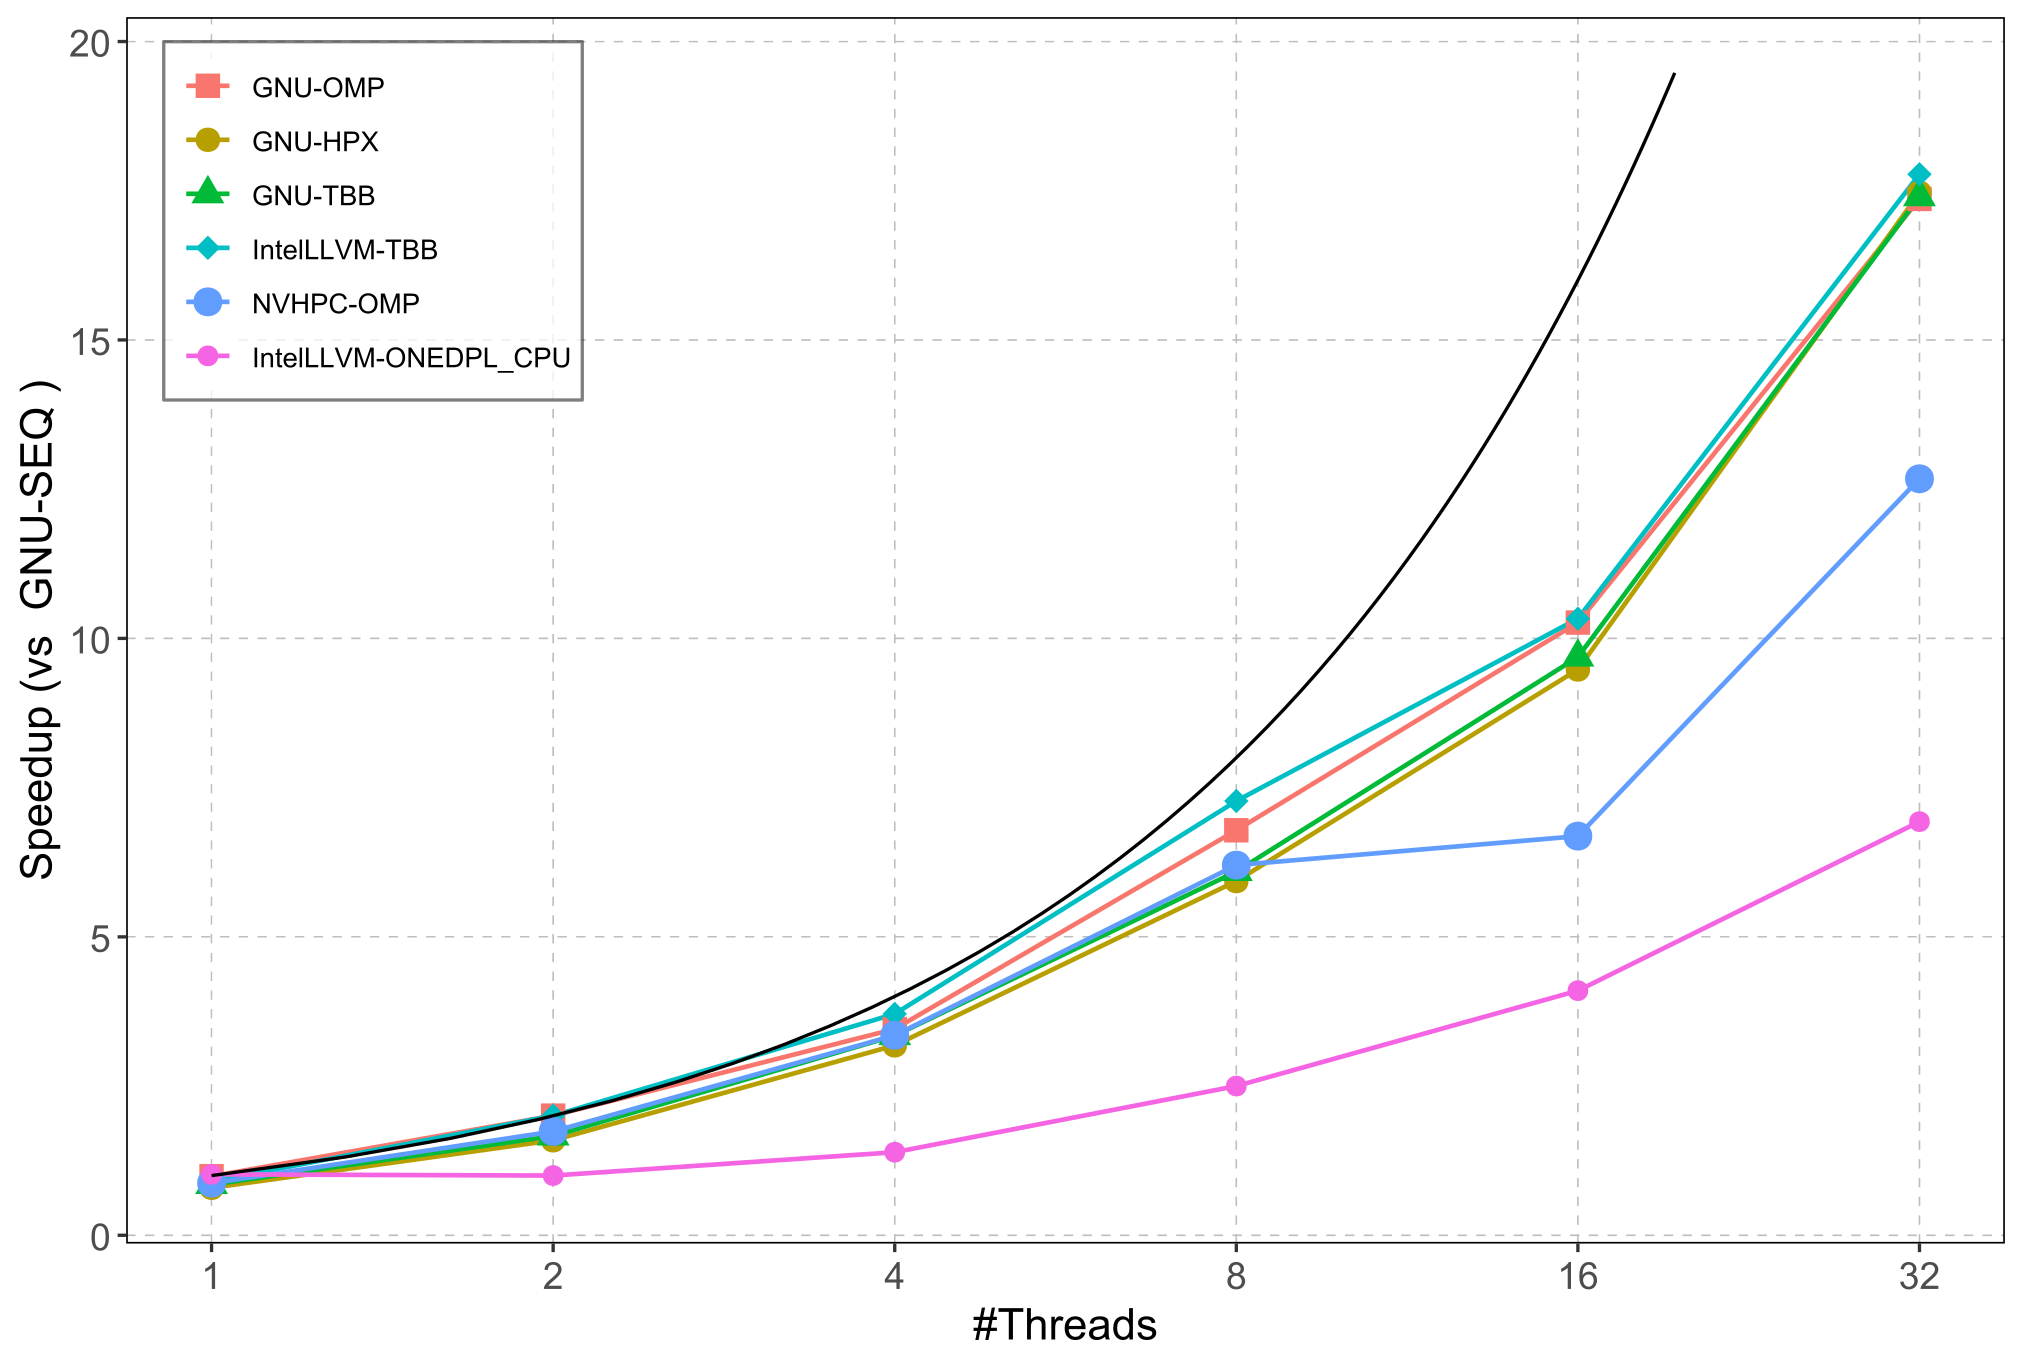
\includegraphics[width=\linewidth]{figures/speedup_threads-for_each-k1000.png}
            \caption*{(b) $k_{it} = 1000$.}
      \end{minipage}
      \caption{Results for benchmark X::for\_each. Strong scaling with $2^{29}$
            elements. Higher is better.}\label{fig:speedup_threads-for_each}
\end{figure}

\subsection{X::find}
The \textit{find} algorithm performs a linear search over a range to locate a
target value.

Figure~\ref{fig:x::find} presents the execution time for the \textit{find}
algorithm. The results are consistent with those reported in the original
pSTL-Bench paper, where sequential execution significantly outperforms parallel
implementations for small problem sizes.

As the problem size increases, parallel backends gradually begin to outperform
the sequential version.

However, the maximum observed speedup remains relatively modest, with the best
performance achieved by the NVIDIA OpenMP backend.

Across all problem sizes, the oneDPL backend on CPU consistently delivered the
lowest performance—even falling below that of the sequential implementation.

\begin{figure}[H]
      \centering
      \begin{minipage}[t]{0.48\linewidth}
            \centering
            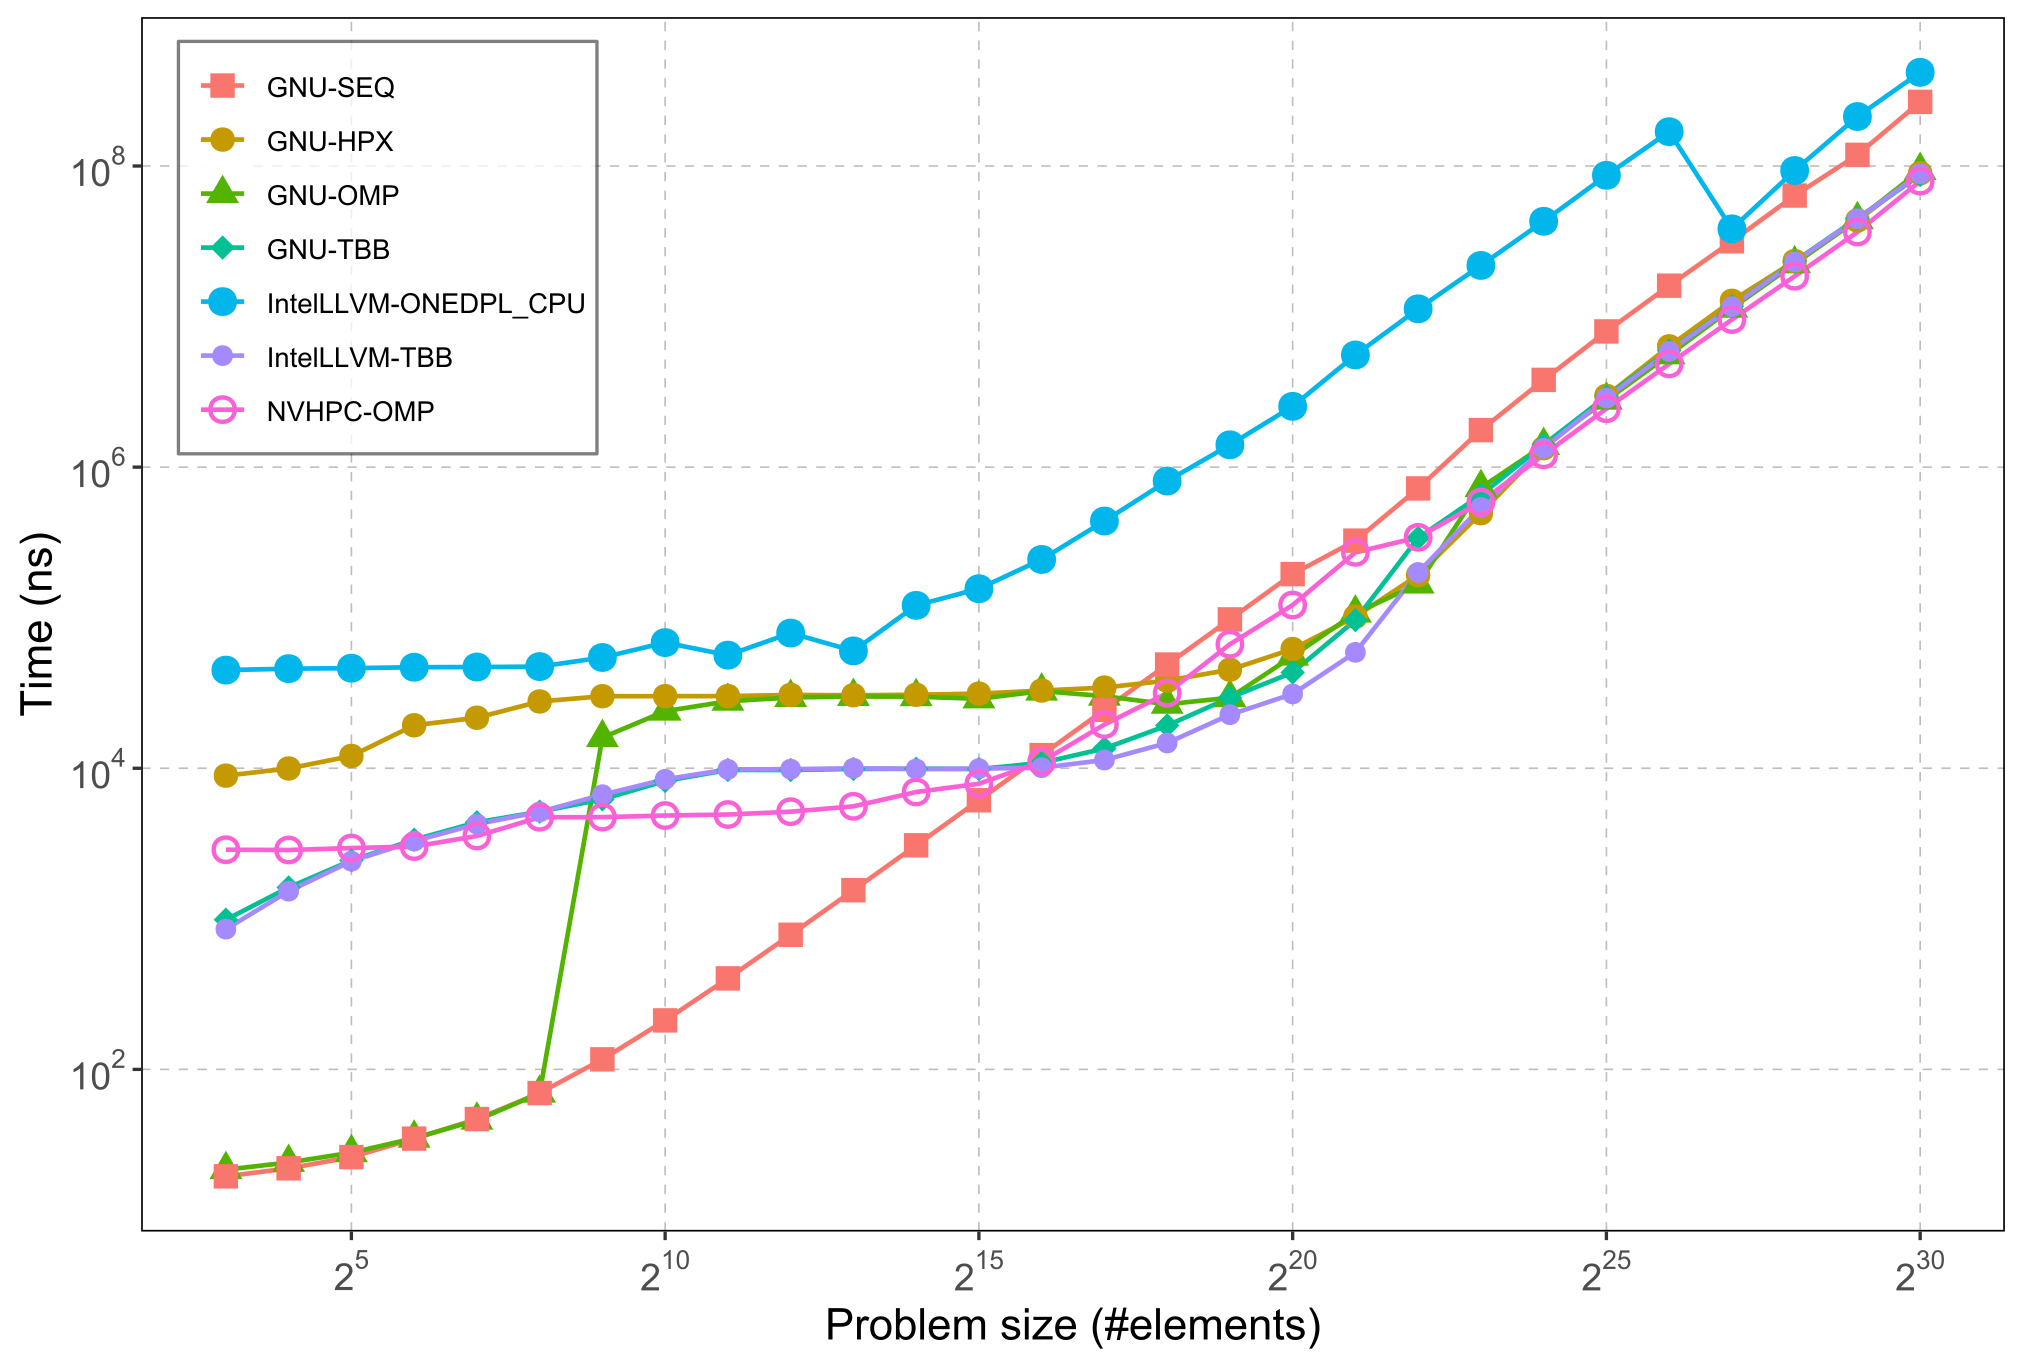
\includegraphics[width=\linewidth]{figures/problemSize_time-find.png}
            \caption*{(a) Problem scaling. Lower is better.}
      \end{minipage}
      \hfill
      \begin{minipage}[t]{0.48\linewidth}
            \centering
            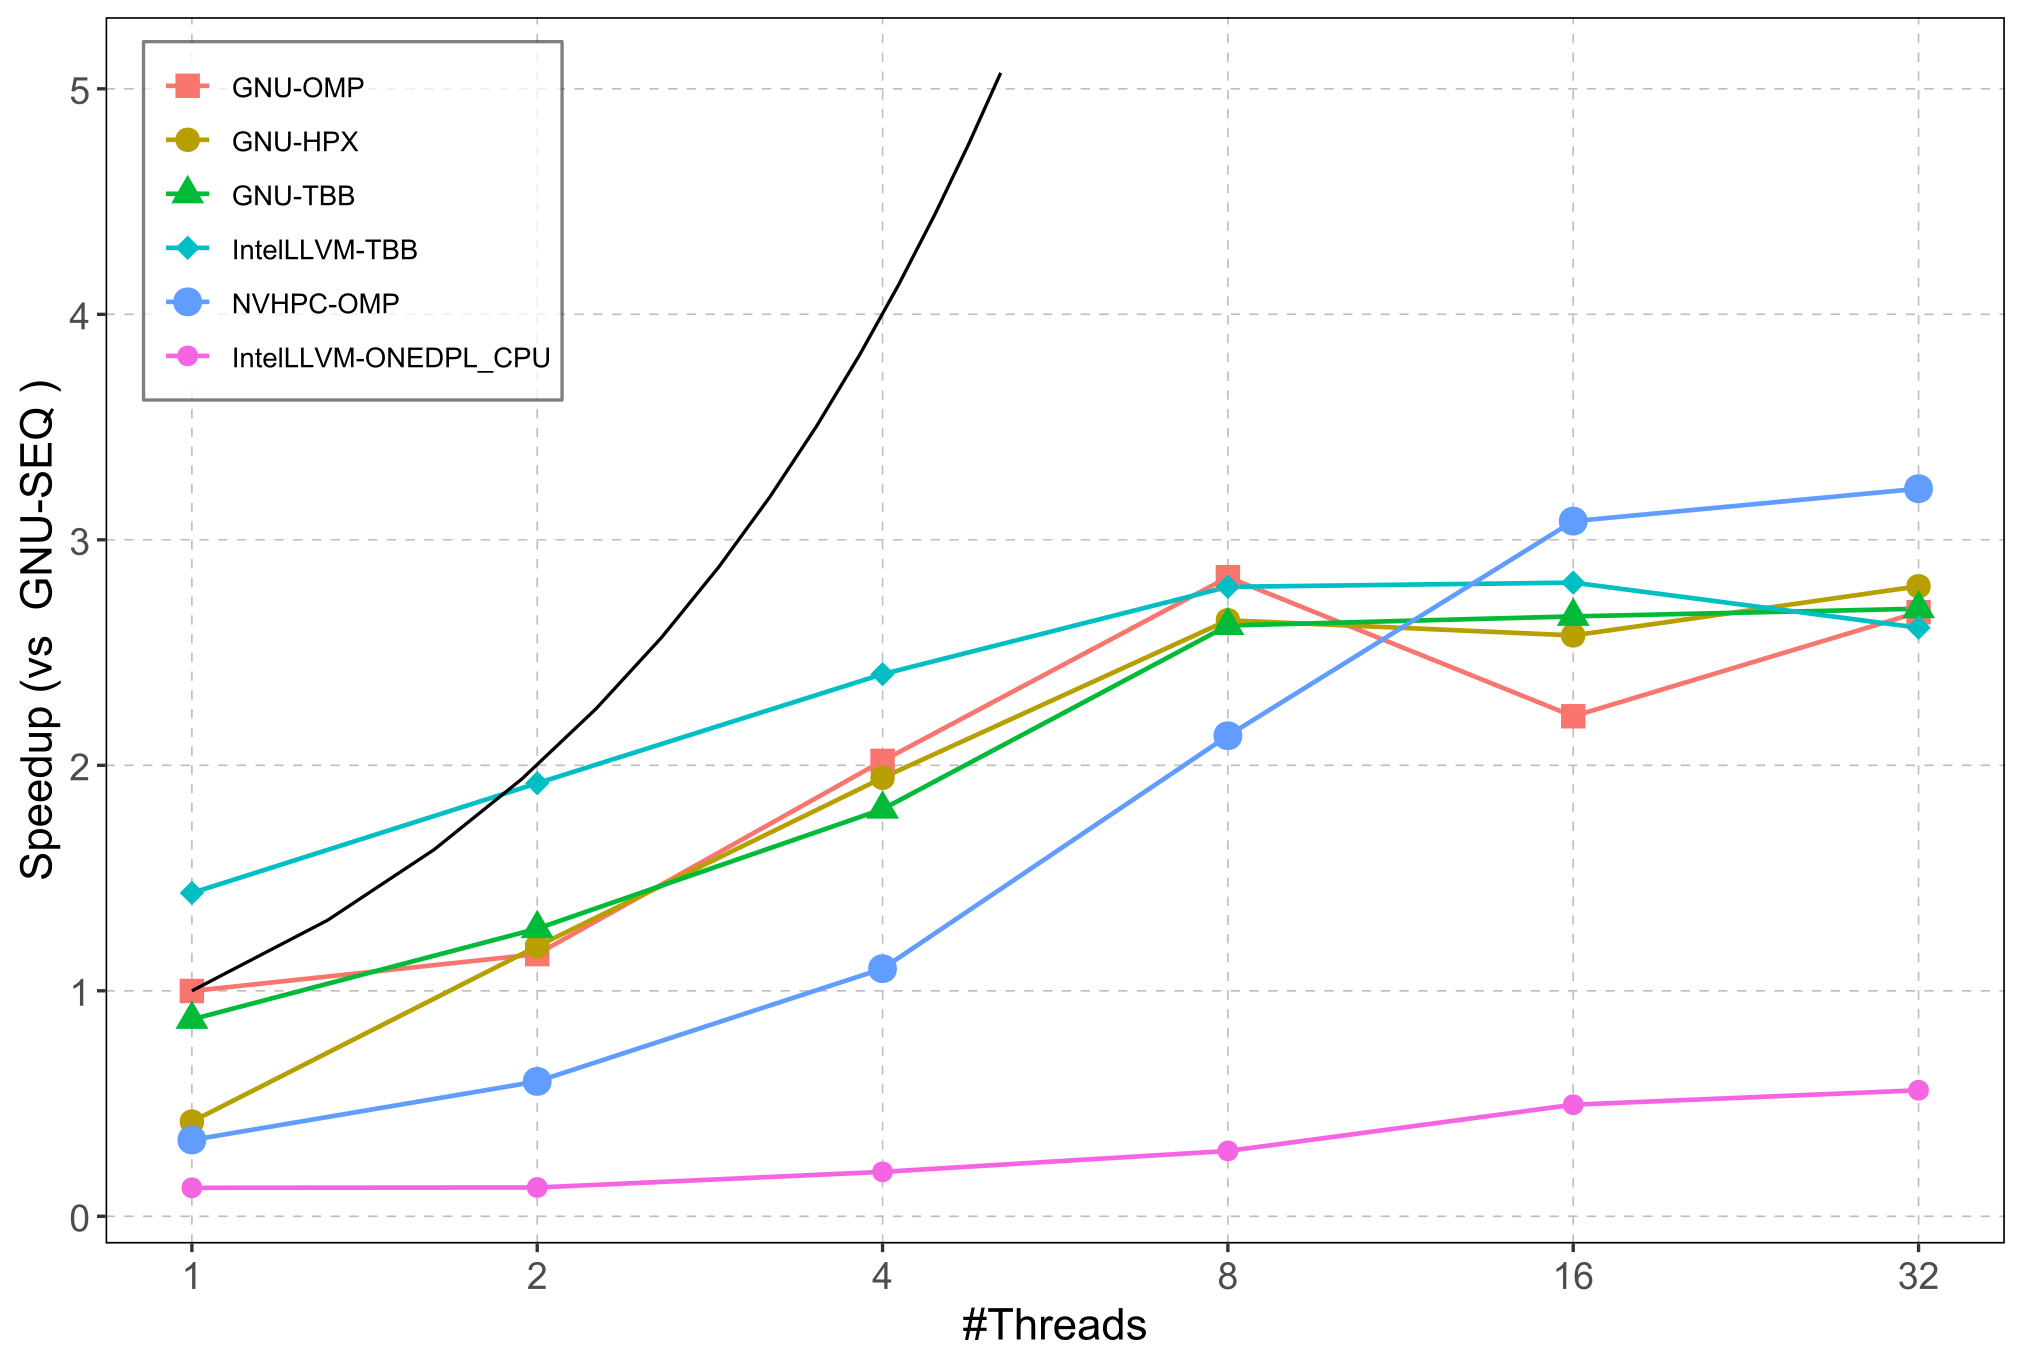
\includegraphics[width=\linewidth]{figures/speedup_threads-find.png}
            \caption*{(b) Strong scaling with $2^{29}$ elements. Higher is better.}
      \end{minipage}
      \caption{Results for X::find.}\label{fig:x::find}
\end{figure}

\subsection{X::inclusive\_scan}

The \textit{inclusive\_scan} algorithm computes a prefix sum, where each
element in the output is the sum of all preceding elements plus the current
element.

The GNU OpenMP implementation is omitted from the results, as it does not
support this algorithm. Although the NVIDIA OpenMP backend also lacks native
support, it falls back to a sequential implementation.

Figure~\ref{fig:x::inclusive_scan} shows the execution time for the
\textit{inclusive\_scan} algorithm. The results are consistent with those in
the original pSTL-Bench paper, where sequential execution significantly
outperforms parallel implementations for small problem sizes.

As the problem size increases, the performance of the parallel backends begins
to approach that of the sequential version, with the TBB implementations
achieving the best results overall.

Observed speedups remain modest and tend to degrade when using more than 8
threads. This decline is likely due to the underlying hardware architecture,
which consists of 8 performance cores (P-cores) and 16 efficiency cores
(E-cores).

Across all problem sizes, the oneDPL backend on CPU consistently exhibited the
lowest performance—even falling below that of the sequential baseline.

\begin{figure}[H]
      \centering
      \begin{minipage}[t]{0.48\linewidth}
            \centering
            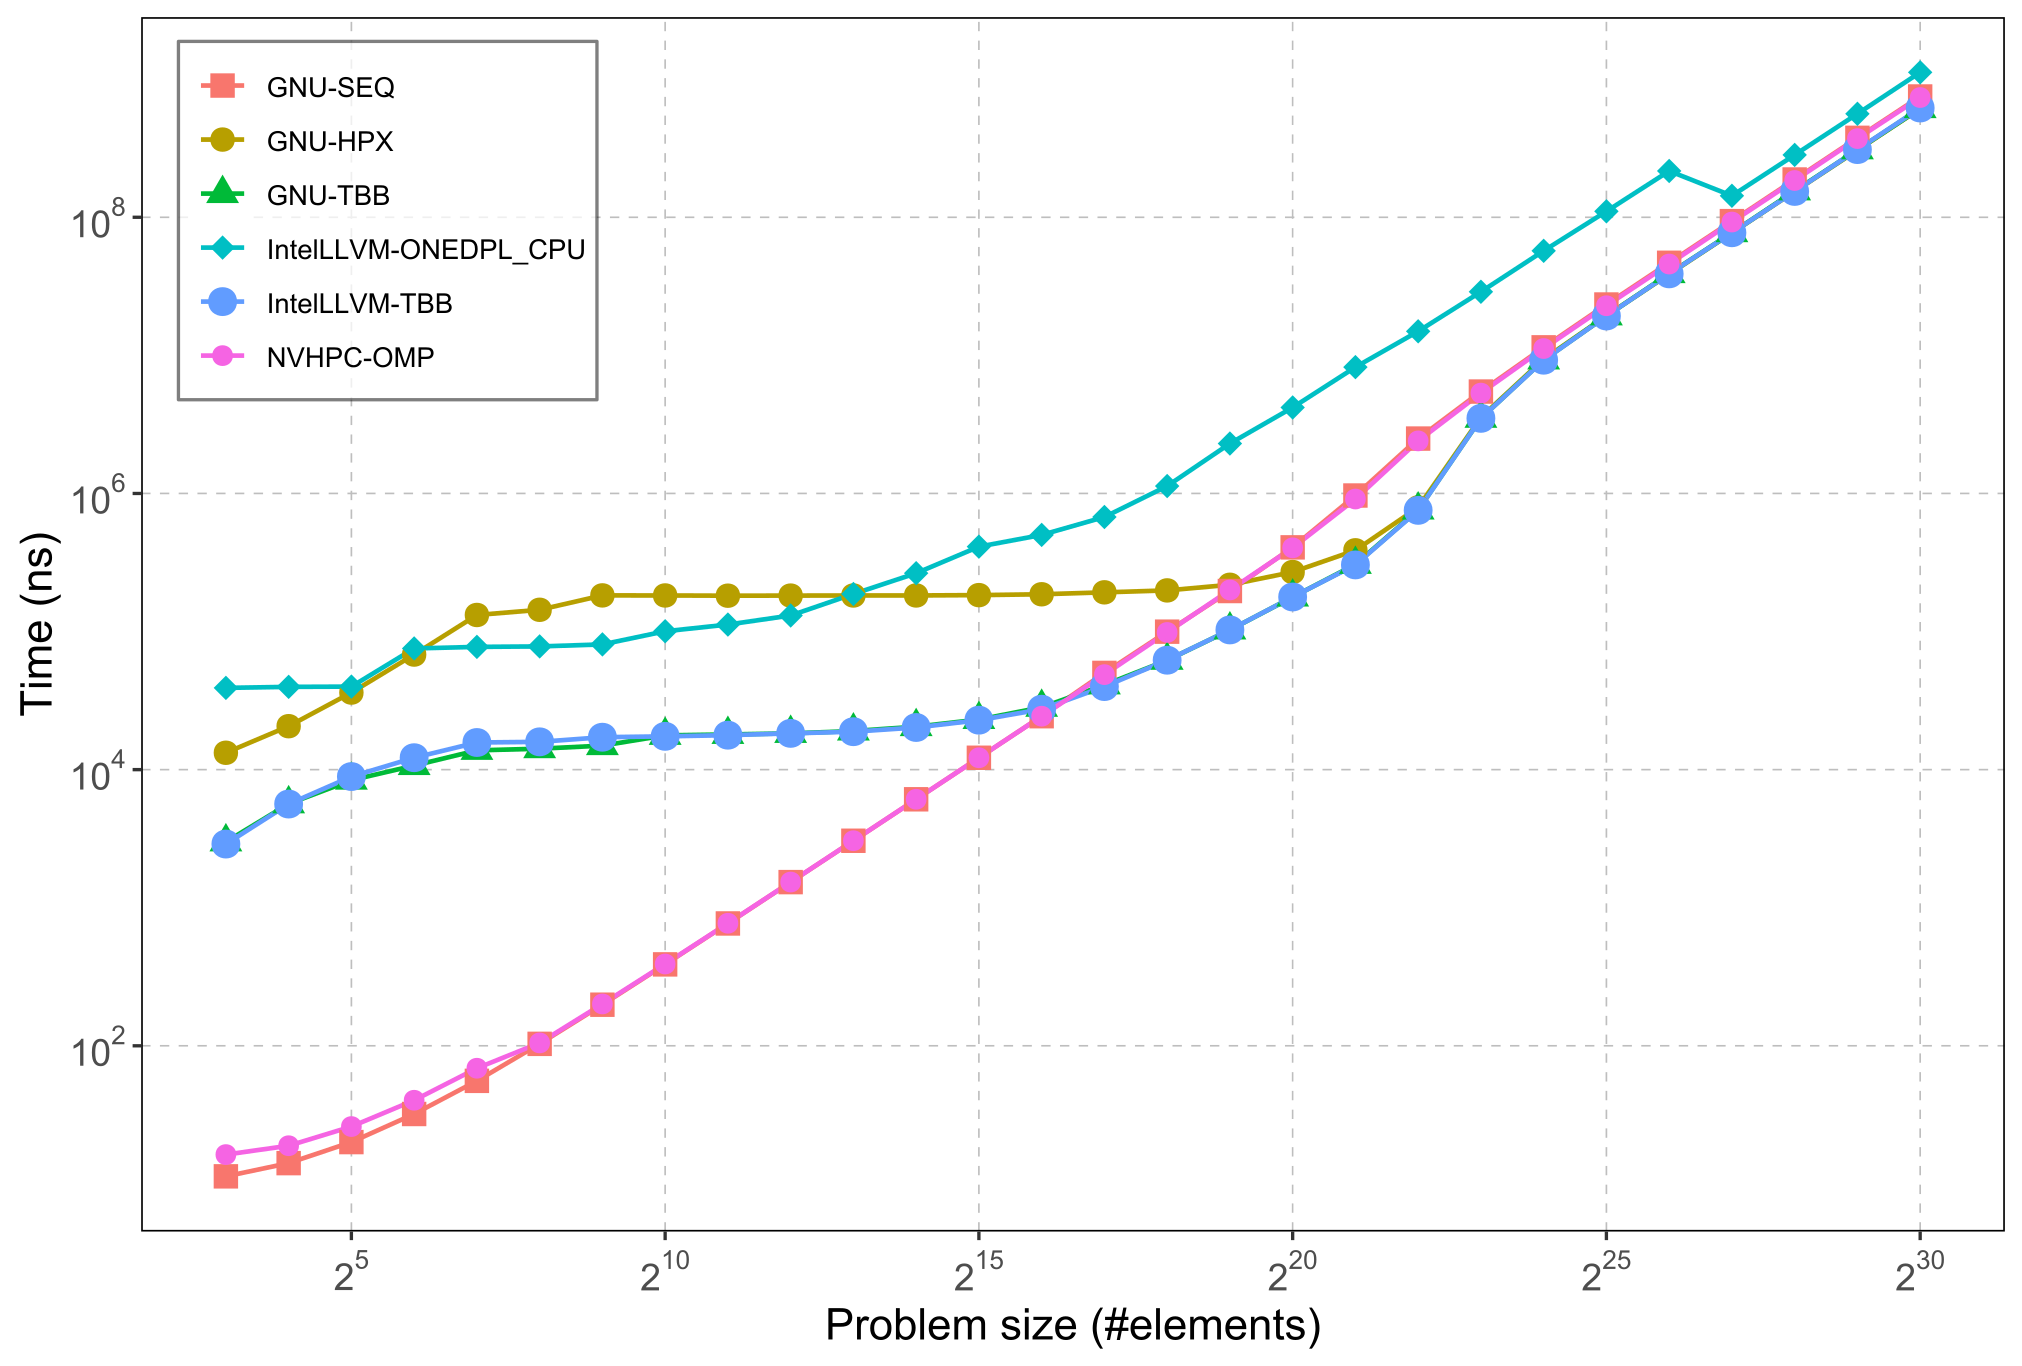
\includegraphics[width=\linewidth]{figures/problemSize_time-inclusive_scan.png}
            \caption*{(a) Problem scaling. Lower is better.}
      \end{minipage}
      \hfill
      \begin{minipage}[t]{0.48\linewidth}
            \centering
            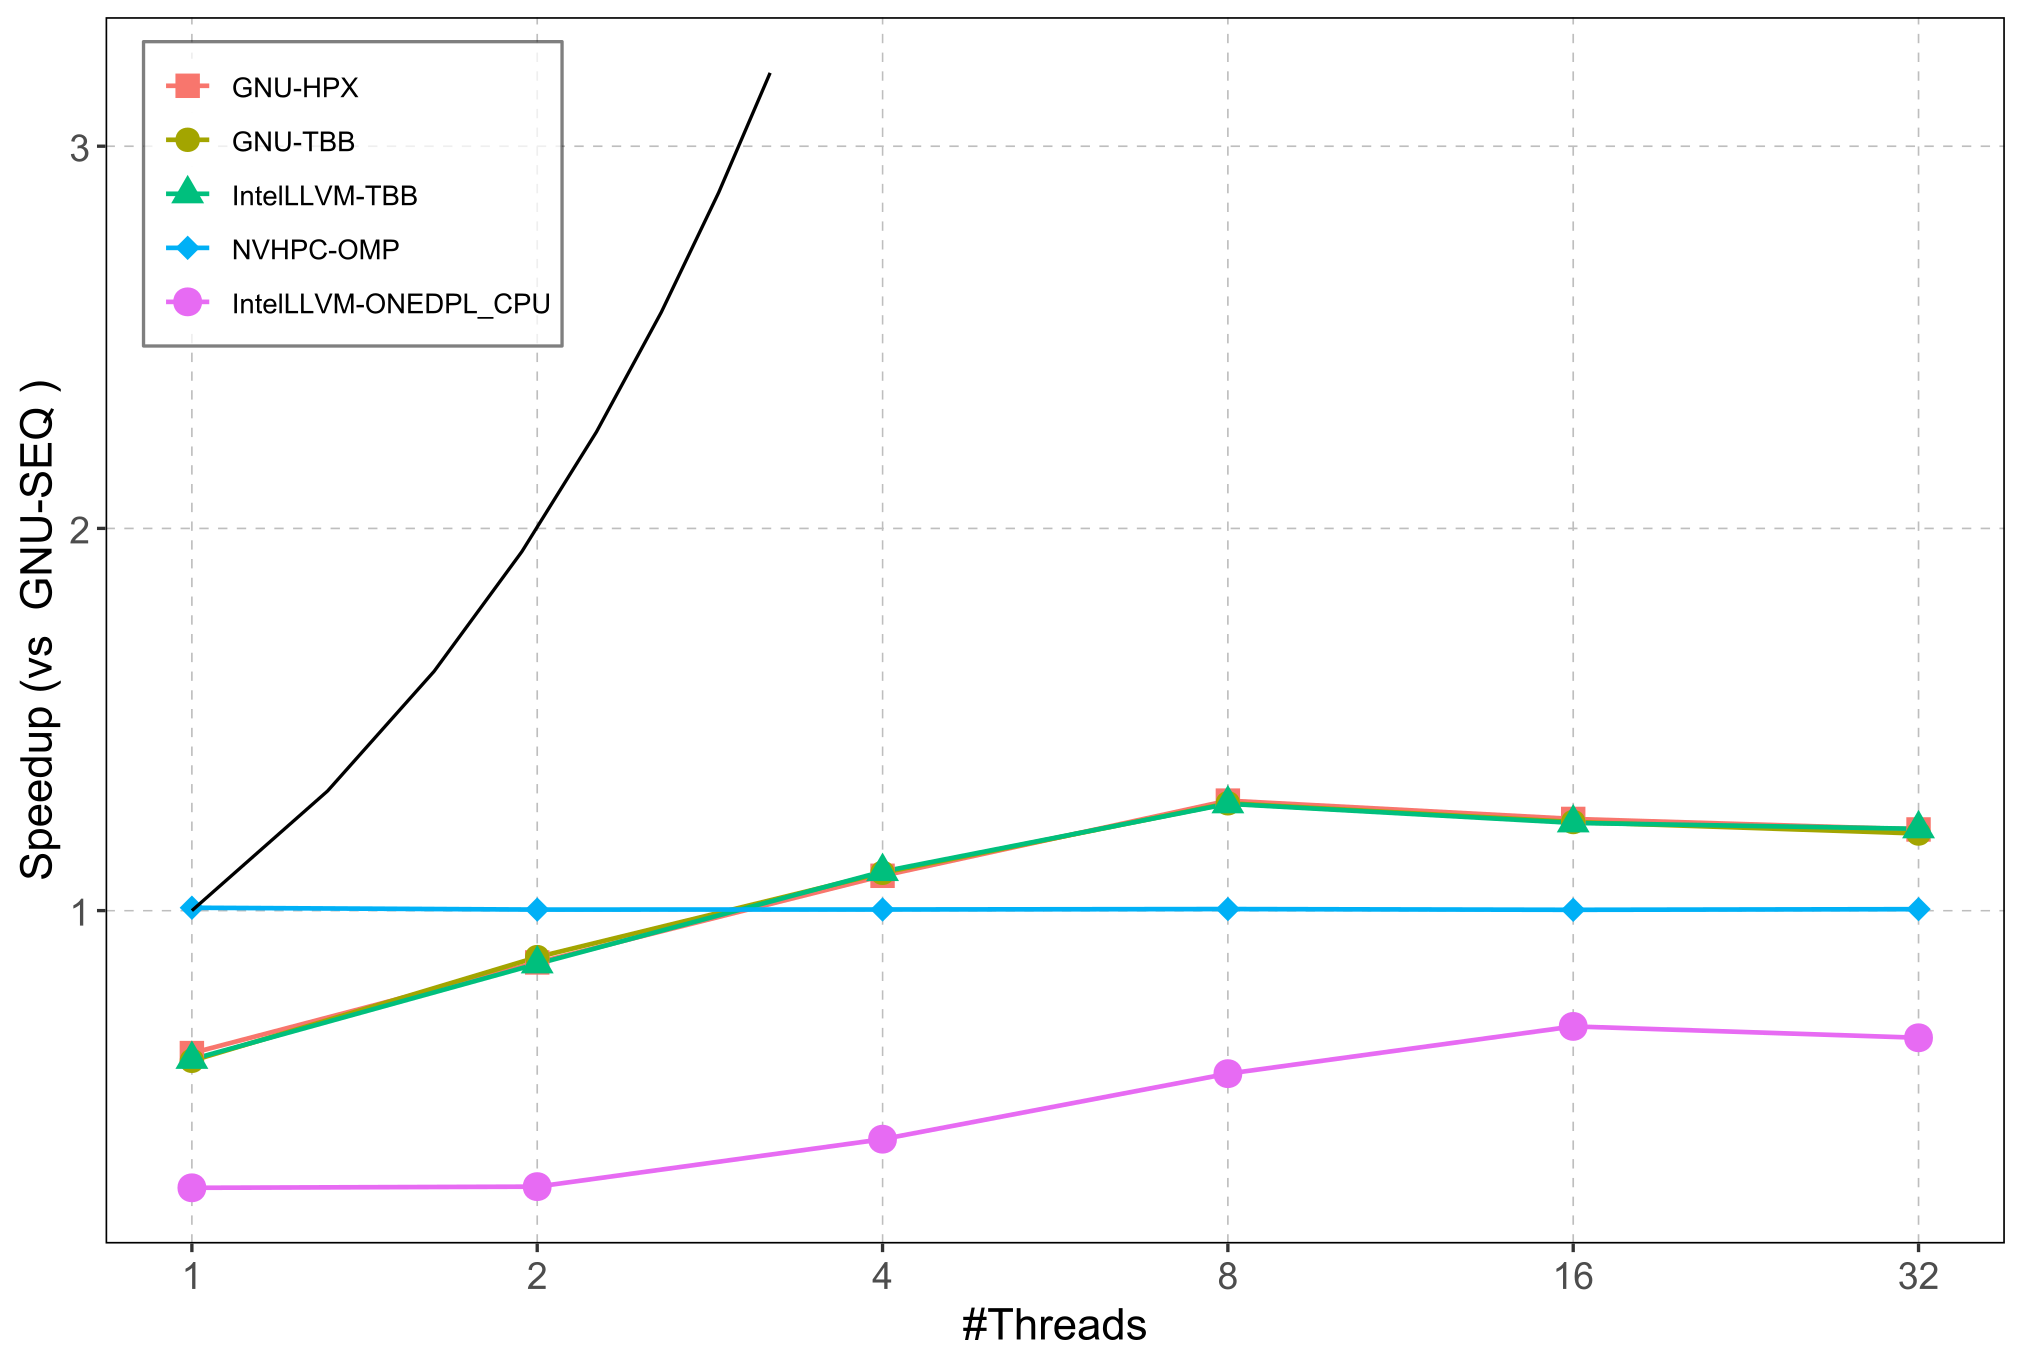
\includegraphics[width=\linewidth]{figures/speedup_threads-inclusive_scan.png}
            \caption*{(b) Strong scaling with $2^{29}$ elements. Higher is better.}
      \end{minipage}
      \caption{Results for X::inclusive\_scan.}\label{fig:x::inclusive_scan}
\end{figure}

\section{Conclusions}

Here you need to summarize what you did and why this is important. {\em Do not
            take the abstract} and put it in the past tense. Remember, now the reader has
(hopefully) read the report, so it is a very different situation from the
abstract. Try to highlight important results and say the things you really want
to get across such as high-level statements (e.g., we believe that .... is the
right approach to .... Even though we only considered x, the .... technique
should be applicable ....) You can also formulate next steps if you want. Be
brief. After the conclusions there are only the references.

\balance{}
\bibliographystyle{ACM-Reference-Format}
\begin{thebibliography}{1}

      \bibitem{pSTL-Bench}
      R. Laso, D. Krupitza, and S. Hunold, ``Exploring Scalability in C++ Parallel STL Implementations'' in \textit{Proceedings of the 53rd International Conference on Parallel Processing (ICPP '24)},
      Association for Computing Machinery, New York, NY, USA, 2024, pp. 284--293.
      \url{https://doi.org/10.1145/3673038.3673065}

      \bibitem{app}
      W. -C. Lin, T. Deakin and S. McIntosh-Smith, ``Evaluating ISO C++ Parallel Algorithms on Heterogeneous HPC Systems'' in  \textit{2022 IEEE/ACM International Workshop on Performance Modeling, Benchmarking and Simulation of High Performance Computer Systems (PMBS)},
      Dallas, TX, USA, 2022, pp. 36-47.
      \url{https://doi.org/10.1109/PMBS56514.2022.00009}

      \bibitem{Kokkos}
      H. C. Edwards and C. R. Trott, ``Kokkos: Enabling Performance Portability Across Manycore Architectures'' \textit{2013 Extreme Scaling Workshop (xsw 2013)},
      Boulder, CO, USA, 2013, pp. 18-24.
      \url{https://doi.org/10.1109/XSW.2013.7}

      \bibitem{RAJA}
      D. A. Beckingsale et al., ``RAJA: Portable Performance for Large-Scale Scientific Applications'' \textit{2019 IEEE/ACM International Workshop on Performance, Portability and Productivity in HPC (P3HPC)},
      Denver, CO, USA, 2019, pp. 71-81.
      \url{https://doi.org/10.1109/P3HPC49587.2019.00012}

      \bibitem{cpu_specs}
      Intel, ``Intel Core i9-13900HX Processor'' \textit{Intel SKU},
      \url{https://www.intel.com/content/www/us/en/products/sku/232171/intel-core-i913900hx-processor-36m-cache-up-to-5-40-ghz/specifications.html}

      \bibitem{gpu_specs}
      NVIDIA, ``GeForce RTX 4070 Laptop GPU'' \textit{GeForce RTX 40 Series Laptops},
      \url{https://www.nvidia.com/en-us/geforce/laptops/40-series/}

      \bibitem{google_benchmark:governor}
      Google Benchmark, ``Reducing Variance, Disabling CPU Frequency Scaling'' \textit{Google Benchmark Documentation},
      \url{https://google.github.io/benchmark/reducing_variance.html}

\end{thebibliography}

\end{document}

